\documentclass[../SpecificaTecnica.tex]{subfiles}
\begin{document}
\section{Componenti e classi}
	\subsection{**NomeApplicazione**}
	Namespace globale dell'applicazione. Le relazioni tra i package Model, View e Presenter rappresentano le relazioni tipiche del design pattern MVP.
		\subsubsection{Package contenuti}
			\begin{itemize}
				\item **NomeApplicazione**::Model;
				\item **NomeApplicazione**::View;
				\item **NomeApplicazione**::Presenter.
			\end{itemize}
	\newpage
	\subsection{**NomeApplicazione**::Model}
		\subsubsection{Struttura del package}
				\begin{figure}[!h]
					\centering
					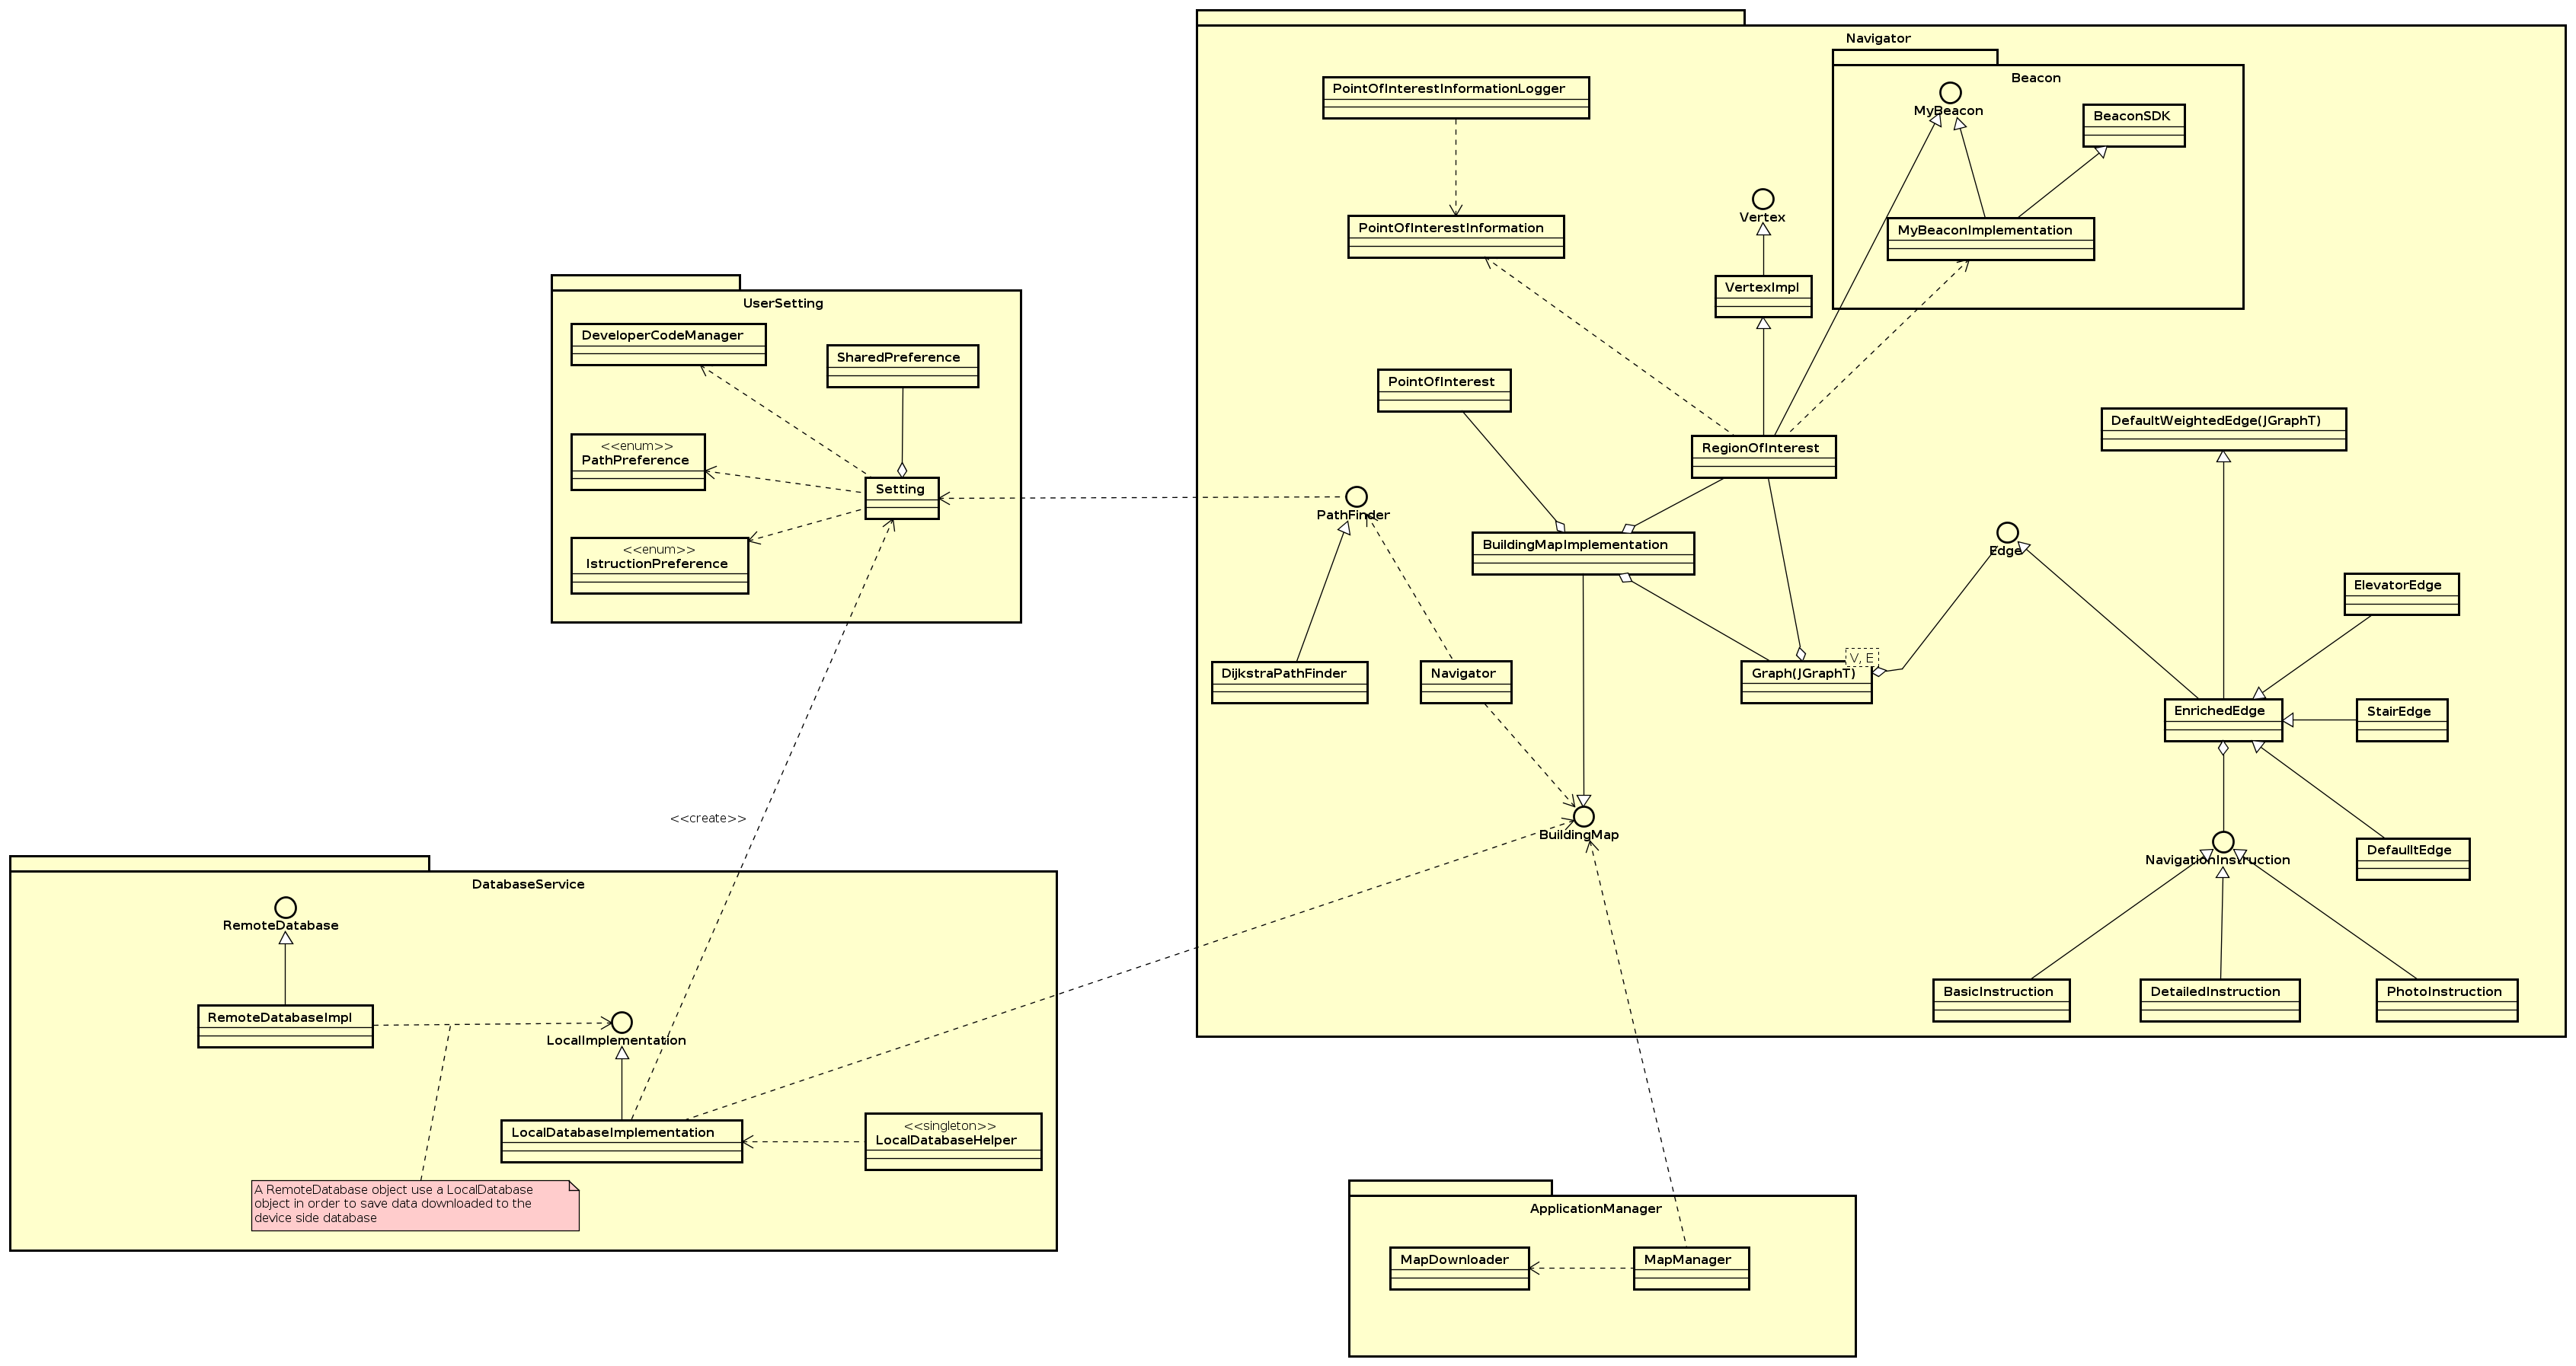
\includegraphics[scale=0.12]{diagrammi/Model.png}
						\caption{Struttura del pacchetto Model}
					\label{fig:Struttura_MVP}
				\end{figure} 
		\subsubsection{Descrizione}
			Package che contiene tutte le classi e package appartenenti al Model dell'applicazione.
		\subsubsection{Package contenuti}
			\begin{itemize}
				\item **NomeApplicazione**::Model::UserSetting;
				\item **NomeApplicazione**::Model::Navigator;
				\item **NomeApplicazione**::Model::Beacon;
				\item **NomeApplicazione**::Model::DatabaseServices
				\item **NomeApplicazione**::Model::ApplicationManager
			\end{itemize}
			\newpage
	\subsection{**NomeApplicazione**::Model::UserSetting}
		\subsubsection{Struttura del package}
			\begin{figure}[!h]
				\centering
				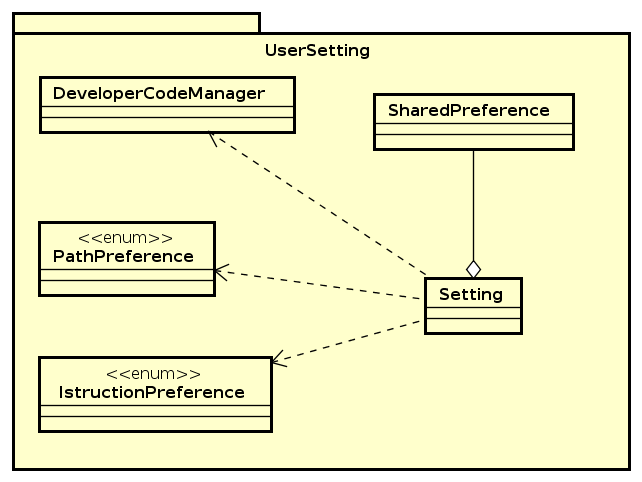
\includegraphics[scale=0.6]{diagrammi/UserSetting.png}
					\caption{Struttura del pacchetto UserSetting}
				\label{fig:Struttura_MVP}
			\end{figure} 
		\subsubsection{Descrizione}
			Componente del Model per la gestione delle preferenze riguardanti il percorso, le impostazioni di fruizione delle informazioni di navigazione e per gestire se un utente può accedere alle funzioni di sviluppatore oppure no.
		\subsubsection{Classi}
			\paragraph{**NomeApplicazione**::Model::UserSetting::Setting}
				Classe per accedere alle impostazioni di un utente. \\
				Viene utilizzata per mantenere un riferimento in memoria e accedere a queste informazioni quando serve(per esempio quando viene effettuato il calcolo del percorso). Le preferenze vengono salvate tramite la classe "SharedPreference" di Android.
			\paragraph{**NomeApplicazione**::Model::UserSetting::PathPreference}
				Classe che definisce le preferenze impostabili riguardanti il percorso preferito dall'utente. \\
				È un semplice enumeratore utile solamente per definire tutti e soli i valori che possono essere utilizzati in **NomeApplicazione**::Model::UserSetting::Setting.
			\paragraph{**NomeApplicazione**::Model::UserSetting::IstructionPreference}
				Classe che definisce le preferenze impostabili riguardanti la fruizione delle istruzioni di navigazione. \\
				È un semplice enumeratore utile solamente per definire tutti e soli i valori che possono essere utilizzati in **NomeApplicazione**::Model::UserSetting::Setting.
			\paragraph{**NomeApplicazione**::Model::UserSetting::DeveloperCodeManager}
				Classe statica per la verifica dei codici sviluppatore. \\
				Questa classe esporrà un metodo pubblico che ricevuta una stringa ritornerà un booleano che specificherà se il codice passato come parametro è valido oppure no. In prima battuta possiamo fare questo controllo hard-coded, con dei raffinamenti invece possiamo mettere sul server i codici sviluppatore.
	\newpage
	\subsection{**NomeApplicazione**::Model::Beacon}
		\subsubsection{Struttura del package}
		\begin{figure}[!h]
			\centering
			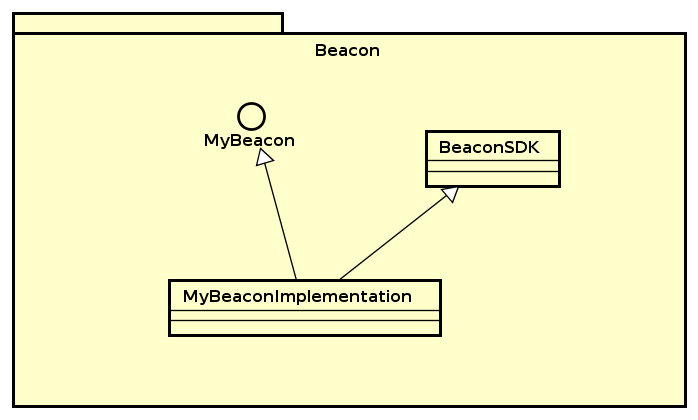
\includegraphics[scale=0.6]{diagrammi/Beacon.png}
				\caption{Struttura del pacchetto Beacon}
			\label{fig:Struttura_MVP}
		\end{figure} 
		\subsubsection{Descrizione}
			Componente del Model per la gestione dei beacon.
		\subsubsection{Interfacce}
			\paragraph{**NomeApplicazione**::Model::Beacon::MyBeacon}
				Interfaccia per accedere alle informazioni di un beacon. \\ 
				Viene utilizzata per specificare il contratto delle classi che la implementano, definendo i metodi che devono essere implementati. Praticamente serve per offrire un livello di astrazione al posto di avere direttamente una classe concreta e quindi poter creare un "adapter" per il beacon della proposto da Altbeacon.
		\subsubsection{Classi}
			\paragraph{**NomeApplicazione**::Model::Beacon::MyBeaconImp}
				Classe che implementa l'interfaccia **NomeApplicazione**::Model::Beacon::MyBeacon. \\
				Questa classe rappresenta un beacon e permette di accedere alle sue informazioni tramite i metodi definiti nell'interfaccia da cui deriva.
	\subsection{**************Manca la parte di rilevamento dei beacon**************}
	\newpage
	\subsection{**NomeApplicazione**::Model::Navigator}
		\subsubsection{Struttura del package Navigator}
		\begin{figure}[!h]
			\centering
			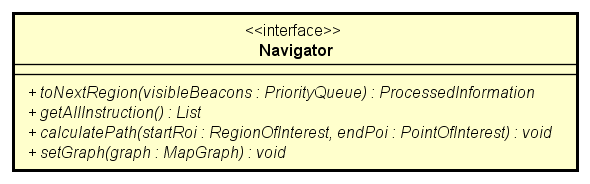
\includegraphics[scale=0.3]{diagrammi/Navigator.png}
				\caption{Struttura del pacchetto Navigator}
			\label{fig:Struttura_MVP}
		\end{figure} 
		\subsubsection{Descrizione}
			Componente del Model che si occupa della parte di navigazione. \\
			Questo pacchetto ha il compito di calcolare il percorso che l'utente deve seguire ed offrire le classi che permettono di rappresentare la mappa.
			\subsubsection{Interfacce}
				\paragraph{**NomeApplicazione**::Model::Navigator::Vertex}
					Interfaccia che rappresenta un vertice di un grafo. \\ 
					Viene utilizzata per dare un livello di astrazione molto alto rispetto a ciò che effettivamente utilizzeremo durante la navigazione. Definisce il contratto di metodi molto semplici come metodi per accedere all'identificativo di un certo vertice.
				\paragraph{**NomeApplicazione**::Model::Navigator::Edge}
					Interfaccia che rappresenta un arco pesato di un grafo. \\ 
					Viene utilizzata per dare un livello di astrazione molto alto rispetto a ciò che effettivamente utilizzeremo durante la navigazione. Definisce il contratto di metodi molto semplici come metodi per accedere al peso dell'arco, ai nodi iniziali e finali dell'arco, impostare i nodi dell'arco.
				\paragraph{**NomeApplicazione**::Model::Navigator::PathFinder}
					Interfaccia che espone il contratto della classe che calcola il percorso. \\ 
					Questa interfaccia viene utilizzata per definire la firma dei metodi per gli algoritmi che possono calcolare il percorso definendo uno "Strategy".
				\paragraph{**NomeApplicazione**::Model::Navigator::BuildingMap}
					Interfaccia che rappresenta la mappa di un edificio. \\
					Viene utilizzata per definire il contratto che le classi devono seguire per poter rappresentare una mappa utilizzabile dal nostro Model.
				\paragraph{**NomeApplicazione**::Model::Navigator::NavigationInstruction}
					Interfaccia che rappresenta le informazioni di navigazione. \\
			\subsubsection{Classi}
				\paragraph{**NomeApplicazione**::Model::Navigator::VertexImp}
					Classe che implementa l'interfaccia **NomeApplicazione**::Model::Navigator::Vertex. \\
					Questa classe rappresenta un vertice e permette di accedere alle sue informazioni tramite i metodi definiti nell'interfaccia da cui deriva.
				\paragraph{**NomeApplicazione**::Model::Navigator::RegionOfInterest}
					Classe che estende **NomeApplicazione**::Model::Navigator::VertexImp e **NomeApplicazione**::Model::Beacon::MyBeaconImp. \\
					Questa classe rappresenta un "punto di navigazione" nel grafo rappresentante l'edificio, ovvero rappresenta un beacon come un vertice nel grafo dell'edificio.
				\paragraph{**NomeApplicazione**::Model::Navigator::EnrichedEdge}
					Classe che implementa l'interfaccia **NomeApplicazione**::Model::Navigator::Edge e deriva dalla classe org.jgrapht.graph.DefaultWeightedEdge della libreria JGraphT. \\
					Viene utilizzata per la navigazione. Infatti questo tipo di arco contiene informazione sia sul peso dell'arco (utile per il calcolo del percorso), sia l'informazioni di attraversamento (informazioni di base, descrizione lunga, url delle photo).
				\paragraph{**NomeApplicazione**::Model::Navigator::ElevatorEdge}
					Classe che estende la classe **NomeApplicazione**::Model::Navigator::EnrichedEdge. \\
					Rappresenta un arco che prevede un ascensore e viene utilizzata per ridefinire il peso utilizzato per calcolare il percorso sulla base delle preferenze dell'utente in base agli ascensori.
				\paragraph{**NomeApplicazione**::Model::Navigator::StairEdge}
					Classe che estende la classe **NomeApplicazione**::Model::Navigator::EnrichedEdge. \\
					Rappresenta un arco che prevede delle scale e viene utilizzata per ridefinire il peso utilizzato per calcolare il percorso sulla base delle preferenze dell'utente in base alle scale.
				\paragraph{**NomeApplicazione**::Model::Navigator::DefaultEdge}
					Classe che estende la classe **NomeApplicazione**::Model::Navigator::EnrichedEdge. \\
					Rappresenta un arco che non contiene particolari ostacoli e viene utilizzata per ridefinire il peso utilizzato per calcolare il percorso nel caso in cui l'utente non imposti alcuna preferenza di percorso.
				\paragraph{**NomeApplicazione**::Model::Navigator::BasicInstruction}
					Classe che implementa l'interfaccia\\ **NomeApplicazione**::Model::Navigator::NavigationInstruction. \\
					Rappresenta le indicazioni di base che possono guidare un utente (Navigazione di primo livello).
				\paragraph{**NomeApplicazione**::Model::Navigator::DetailedInstruction}
					Classe che implementa l'interfaccia\\ **NomeApplicazione**::Model::Navigator::NavigationInstruction. \\
					Rappresenta delle informazioni aggiuntive che possono essere fornite ad un utente (descrizione lunga).
				\paragraph{**NomeApplicazione**::Model::Navigator::PhotoInstruction}
					Classe che implementa l'interfaccia\\ **NomeApplicazione**::Model::Navigator::NavigationInstruction. \\
					Rappresenta delle informazioni visuali del prossimo punto da raggiungere per procedere con la navigazione (fotografie).
				\paragraph{**NomeApplicazione**::Model::Navigator::PointOfInterest}
					Classe che rappresenta un POI ovvero un area dell'edificio che può risultare interessante ad un utente a livello sia informativo che di navigazione (una possibile destinazione). \\
					Questa classe offre la possibilità di accedere alle informazioni di un POI quali:
					\begin{itemize}
						\item nome del POI (esistente o dato da noi);
						\item descrizione del POI (qualcosa che almeno ne descriva le funzionalità);
					\end{itemize}
				\paragraph{**NomeApplicazione**::Model::Navigator::BuildingMapIml}
					Classe che implementa l'interfaccia **NomeApplicazione**::Model::Navigator::BuildingMapImplementation. \\
					Viene utilizzata per rappresentare la mappa dell'edificio, racchiudento le informazioni dell'edificio stesso. in particolare mantiene la corrispondenza tra RegionOfInterest e PointOfInterest (ad un ROI possono essere associati più POI ed un POI può appartenere a più ROI. Esempio 1C150 della Torre Archimede). 
				\paragraph{**NomeApplicazione**::Model::Navigator::DijktraPathFinder}
					Classe che implementa l'interfaccia **NomeApplicazione**::Model::Navigator::PathFinder. \\
					Viene utilizzata per calcolare il percorso per portare un utente in un certo POI (destinazione della navigazione). Questa classe sfrutta gli algoritmi messi a disposizione dalla libreria JGraphT. Essendo che un POI può essere associato a più ROI e la navigazione è possibile solamente tramite i ROI (punti in cui abbiamo i beacon e quindi possiamo controllare se l'utente va nel percorso giusto oppure no) allora sarà necessario calcolare un percorso per ogni ROI associato ad un POI e successivamente scegliere quello con peso minore (in base al percorso stesso e alle preferenze dell'utente). Utilizzando l'algritmo di Dijkstra non sarebbe necessario in generale ma l'implementazione fornita da JGraphT richiede un ricalcolo.
				\paragraph{**NomeApplicazione**::Model::Navigator::Navigator}
					Classe che si occupa di gestire la navigazione. \\
					Viene utilizzata per controllare se l'utente segue le indicazioni fornite per la navigazione e gestire in generale i percorsi restituiti da Dijkstra (liste di archi, nel nostro caso possibilmente sarebbe meglio EnrichedEdge).
	\subsection{Dubbi \& ToDo}
		\begin{itemize}
			\item manca la parte del model riguardante il rilevamento dei beacon;
			\item manca la parte del model riguardante database e server;
			\item manca la parte del model riguardante le fotografie e la loro gestione;
			\item verifica della parte del model riguardante la gestione del codice sviluppatore;
			\item manca la parte del presenter;
			\item manca la parte della view;
			\item da valutare se il package Beacon è interno o esterno al package Navigator;
			\item da valutare se le informazioni dell'edificio sono una classe separata da BuildingMapIml;
			\item da valutare la gestione dei valori dei beacon che cambiano velocemente.
		\end{itemize}
\end{document}